\chapter{Background}
\label{chap:background}
%----------------------------------------------------------------------------------------
This chapter provides an overview of the main concepts and technologies on which it is based this thesis. \Cref{sec:AC} introduces the Aggregate Computing paradigm; it discusses its core idea, the theory and basic mechanism under it, and finally presents Protelis, a language rooted in this paradigm. 
\Cref{sec:LoRaWAN} introduces the LoRaWAN network protocol, 
finally \Cref{sec:DingNet} introduces the DingNet LoRaWAN network and the relative simulator. 

\section{Aggregate Computing}
\label{sec:AC}
Recent technological developments led to computational and networking capabilities being more and more integrated with everyday objects, such as smartphones, wearable devices, drones, smart vehicular systems, domestic appliances, and other kind of sensors and actuators.
% 
This development led to distributed systems counting many devices differing from each other for computational capabilities and communication technologies, and producing pervasive heterogeneous and complex systems.
% 
The classic approach for distributed systems proposes a device-centric point of view.
% 
The goal is to obtain the global behaviour as emergent phenomena from the interaction of single devices. 
% 
So the focus of the designer is on local structure, behaviour, and interaction. 
% 
The final result is typically a system strongly dependent on communication technology that tends to be rigid and costly to testing, evolve, and maintain.
 
Aggregate computing is an emerging programming paradigm devoted to modern distributed systems~\cite{BealIEEEComputer2015}, which proposes a paradigm shift. 
% 
It proposes to program the entire set of devices as a single entity.
% 
The goal is to define the global behaviour in a declarative way focusing on manipulation of global spatial and temporal data structures. This allows the designer to abstract from the real device that will execute the program, its communication capability, network infrastructure, and its execution platform~\cite{ViroliUbiComp2016}. 
% 
The final result will be a complex, modular, extendible, self-adaptive and self-organized distributed system.
% 
The aggregate computing approach offers base functionalities that are composable with each other to assemble advanced and user-friendly APIs. 
In order to organize all the provided functionalities, a multilayer stack has been designed, which collects them all by abstraction level. 
As it is possible to see from the stack in \autoref{fig:ACstack}, the base constructs are based on the field calculus~\cite{Audrito2019} theory.

\begin{figure}[h]
    \centering
    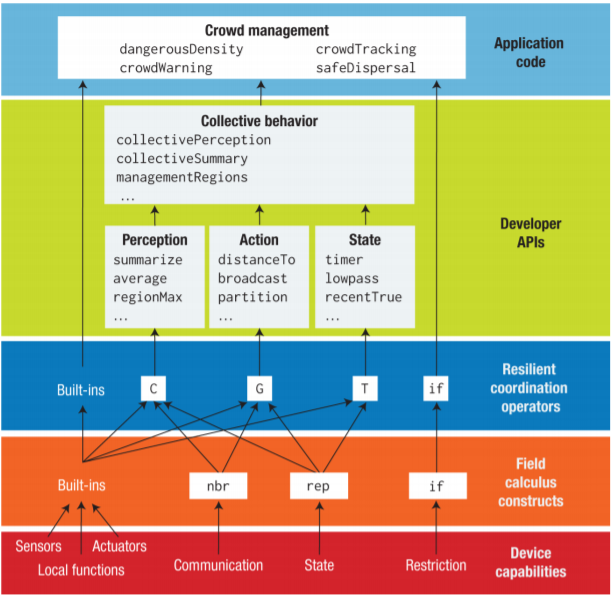
\includegraphics{figures/ACstack.png}
    \caption[Aggregate programming stack]{Aggregate programming stack.~\cite{BealIEEEComputer2015}}
    \label{fig:ACstack}
\end{figure}

\subsection{Field-calculus}

The field calculus is a theoretical model that describes a set of primitives to manipulate the concept of computational field. A computational field is a distributed data structure that maps every networked device to some local value. In field calculus, everything is a field (value, variable, expression, function) and the constructs to build and manipulate it are:
\begin{itemize}
    \item \textbf{Functions}, $b(e1,\dots,e_n)$ applies function $b$ to arguments $e1,\dots,e_n$. The output field is obtained by the point-wise evaluation of the operator to the input fields
    \item \textbf{Stateful computation}, $rep(x \leftarrow v)~\{s1; \dots ; s_n\}$ a local variable $x$ is defined and initialized to value $v$. Then the value is periodically updated with the result of statements $s1; \dots ; s_n$
    \item \textbf{Interaction}, $nbr(s)$ share the local value of $s$, represented as a field, with its neighbours. The result is a field of fields (the same information shared from neighbours) that is possible to reduce to a simple field using \textit{hood} operators
    \item \textbf{Domain restriction}, $if(e)~\{s1; \dots ; s_n\}~else~\{s'_1; \dots ; s'_n\}$ split the field in two sub-field according to the evaluation of $e$. Where $e$ is true is applied the statement $s1; \dots ; s_n$, while where $e$ is false is applied the statement $s'_1; \dots ; s'_n$.
\end{itemize}

The behaviour of aggregate systems can be expressed as a functional composition of operators that manipulate (evolve, combine, restrict) computational fields~\cite{type-sound}.

\subsection{Building blocks operators}
Basic field calculus constructors are low-level operators which do not guarantee to develop self-stabilizing programs as proved in~\cite{DBLP:journals/corr/abs-1711-08297}.
In complex system, self-stabilizing property guarantees that after each transitory phase, the system returns to a stationary state (if exists), where it is possible to predict its behaviour. 
\cite{buildingBlock} introduces a set of building block that are programs write with the low-level operators.
These programs are self-stabilizing and it is possible to prove that programs write combining only these functions will be self-stabilizing.
These building blocks compose the central layer of the aggregate programming stack, \autoref{fig:ACstack}, and the main ones are:

\begin{itemize}
    \item $G(source, init, metric, accumulate) \rightarrow$ function to spread information across space. First, build a field of the shortest path that starts from the $source$ with the chosen $metric$. Then spread the information across the field starting from the $init$ value and modifying it at each step with the $accumulate$ function
    \item $C(potential, reduce, local, null) \rightarrow$ function to accumulates $local$ value along the $potential$ field until the source. The final value is obtained applying the $reduce$ function to the $local$ value of the crossed nodes. If there is nothing to accumulate default value $null$ is returned
    \item $T(init, zero, decay)  \rightarrow$ function to evolve the state for a specified period. The period starts from $init$ and decreases to $zero$ with a $decay$ rate
    \item $S(grain, metric)  \rightarrow$ function to split the network into partitions of nodes. This function leverages the $metric$ function to define partitions of a size proportional to $grain$ and elects a leader for each one.
\end{itemize}

This set of four functions with the domain restriction operator is able to provide most of the commonly used coordination patterns for distributed systems. 

\subsection{Protelis}
\label{subSec:Protelis}
Protelis~\cite{PianiniSAC2015} is a language rooted on the aggregate computing paradigm, sharing its semantic with field calculus and inspired on Proto~\cite{Proto}. %
It provides an implementation of the entire aggregate computing stack, and supports for higher-order field calculus~\cite{Audrito2019}, that introduces functions as first-class citizens with a lot of benefits.
Protelis adopts a C- or Java-like syntax to reduce learning curve, but it is a purely functional language.
% Protelis punta ad essere un linguaggio  che consente di utilizzare in modo pratico i principi dell'aggregate computing 
% essendo il costo di riscriversi tutte li librerie molto alto quello che decide di fare è di appoggiarsi suula piattaforma java già esistente cercando di essere quanto più possibile interopoerabile in modo da sfruttare le sue librerie che possono già essere reperite
% 
Protelis aims to be a language that allows to use the principal of the aggregate computing in a practical way. 
It tries as much as possible to be interoperable leaning on the existing Java platform.
This allows to avoid to rewrite aggregate computing libraries for different platforms, and to use the plethora of Java libraries.
According to the aggregate programming languages principles a Protelis program abstracts from the implementation of device capabilities, real network topology and communication technology. 
In order to fill this abstraction gap Protelis requires the implementation of a back-end that provides a platform operation for every node in the system. 
A Protelis backend requires to implement:
\begin{itemize}
    \item \textbf{the device model}, it has to display its sensors, actuators, and capabilities provided by the hardware;
    \item \textbf{the communication layer}, it has to perform two tasks: define the neighbourhood policy, and deliver the messages of each device to the others ones in its neighbourhood. 
\end{itemize}

\clearpage
\section{LoRaWAN}
\label{sec:LoRaWAN}

In the context of smart-city and more in general of the IoT, it is important to have devices able of long-range communications, low battery consumption, and have the lowest possible installation, maintenance, and purchase costs.
Low-power wide-area network~\cite{Raza2017} (LPWAN) is a type of wireless networks that allows to satisfy the first two requirements.
Typically devices for this type of networks can communicate in a range spanning from a few hundred meters in urban areas to over 10 Km in open-spaces areas.
These networks do not only allow to satisfy the first two requirements, but they also contain the costs as composition of three factors:
\begin{itemize}
    \item lightweight protocols, which allow for using devices with simple hardware and cheap;
    \item use of licence-free band frequency with no cost for network occupation;
    \item low power consumption allowing devices to run for years with a small battery.
\end{itemize}

LoRaWAN~\cite{loraalliancetechnicalcommittee2020} is one of the main LPWAN protocol.
A LoRaWAN network, \autoref{fig:LoRaNetwork}, is composed of three fundamental elements: end-devices (aka motes), gateways (aka concentrators) and a network-server. 
% 
The network topology typically is a star-of-stars topology with the gateway that intermediates between motes and network-server.
% 
The communication between gateway and network-server is IP-based, while the communication between gateways and motes uses the LoRa (Long Range) modulation.

\begin{figure}[h]
    \centering
    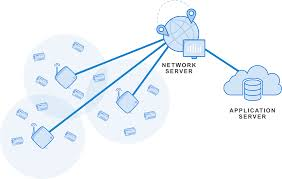
\includegraphics{figures/lora_architecture2.png}
    \caption[LoRaWAN network architecture]{LoRaWAN network architecture~\cite{muntasirjoarder2020} with all the fundamental elements. Straight lines represent IP-based communication, while the circle around the gateways is the communication range based on LoRa modulation.}
    \label{fig:LoRaNetwork}
\end{figure}

The role of network-server is to govern and optimise the interactions between motes and gateways and provides the mote's packet to applications in the application server.
% 
So among other tasks, it has to filter duplicated packet received from gateways and find the best gateway to deliver an application message to a mote.
% 
The LoRaWAN protocol, \autoref{fig:LoRaStack}, is composed of two layers: the  physical layer and the MAC one.

\begin{figure}[h]
    \centering
    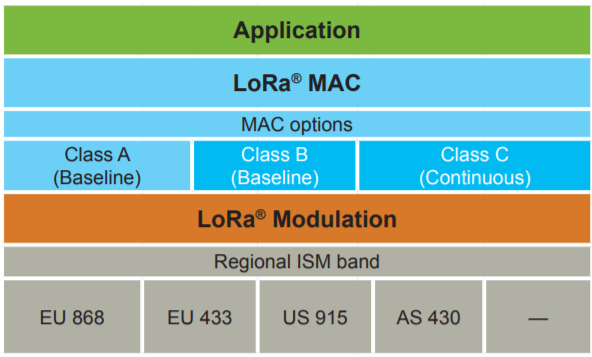
\includegraphics{figures/loraStack.png}
    \caption[LoRaWAN protocol stack]{LoRaWAN protocol stack~\cite{loraalliance2020} where brown rectangle represent the physical layer and the azures rectangles the MAC one.}
    \label{fig:LoRaStack}
\end{figure}

\subsection{Physical Layer}
The physical layer implements the LoRa protocol allowing communication until 15 Km of distance, with a data rate from 0.3 Kb/s to 11 Kb/s with LoRa modulation, and to 50 kb/s with FSK modulation.
% 
The most important parameters for LoRa modulation are Bandwidth (BW), Spreading Factor (SF) and the Code Rate (CR).
% 
The SF value is in the range from 7 to 12 and represents the number of bits in each symbol.
% 
It is an important parameter because define: the maximum packet length, the range of communication, and the bit rate.
% 
SF7 means longest packet length and highest bit rate, but shortest communication range; while SF12 means shortest packet length and lowest bit rate, but longest communication range.
% 
Another important aspect of SF is that concurrent transmissions with different SF will not produce any collision between them.
% 
Finally, LoRa uses the regional Industrial, Scientific and Medical (ISM) band. This means low network cost, but limitation of the duty \mbox{cycle} to maximum 1\% for each channel imposed from the European telecommunications standards institute (ETSI).

\subsection{MAC Layer}
% (Class A, B and C)
The MAC layer regulates the communications between motes and gateways.
% 
Uplink communication (mote to gateways) uses an ALOHA-like protocol. Motes start a broadcast communication when they need without checking the channel state, but applying a small random delay.
% 
For downlink communication (gateway to mote), in order to reduce the battery consumption of the motes, and respect latency requirement of different applications, the layer defines three different classes of devices (A, B and C) with different behaviour.
% 
Devices of class A define two fixed receiving windows after each uplink communication, with the second one opened only if the mote receives a communication during the first. 
% 
This class has the lowest battery consumption with the drawback of the highest latency. 
% 
Devices of class B allow to define more receiving windows, but it is necessary to keep motes and server synchronised via synchronised Beacons. 
% 
This class has lower latency than class A but also higher battery consumption. 
% 
Finally, devices of class C allow always to receive messages except when they execute an uplink communication. 
% 
This class has the lowest latency, but the highest battery consumption.

\section{DingNet: a LoRa-over-MQTT network and simulator}
\label{sec:DingNet}
The LoRaWAN protocol does not standardise communications after the gateways, but defines only that are IP-based.
% 
LoRa-over-MQTT identifies a network where the communication between gateways and network-server is implemented using the public-subscribe pattern via MQTT protocol, and the application server provides data to applications in different ways, but at least via MQTT.
% 
An example of LoRa-over-MQTT architecture is ChirpStack\footnote{\href{https://www.chirpstack.io/}{https://www.chirpstack.io/} (Jan 2020)}, see \autoref{fig:ChirpStack}, that is an open-source LoRaWAN Network Server stack to manage all the LoRaWAN network components and provides data to applications in several ways.

\begin{figure}[h]
    \centering
    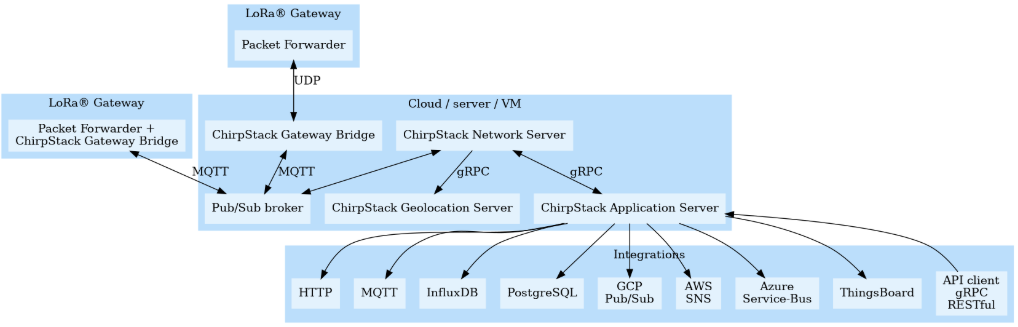
\includegraphics[width=\textwidth]{figures/chirpstack.png}
    \caption[LoRa-over-MQTT architecture]{Example of the LoRa-over-MQTT architecture of ChirpStack.~\cite{chirpstack2020}}
    \label{fig:ChirpStack}
\end{figure}

DingNet\footnote{\href{https://admin.kuleuven.be/icts/english/services/dingnet}{https://admin.kuleuven.be/icts/english/services/dingnet} (Jan 2020)} is a real LoRaWAN network of class A composed of 11 gateways that cover the entire city of Leuven and adopts a LoRa-over-MQTT architecture. 
% 
DingNet allows adding users' devices and applications to the network for research purposes.
% 
The DingNet Simulator~\cite{inproceedings} allows for simulation of applications in different scenarios before deploying them in the real network reducing costs and time for the deployment.
% 
It is a time-driven simulator focused on the simulation of LoRa communications between gateways and motes while the remainder of the network is simulated with a higher-level of abstraction. 
% 
The simulator allows configuring the environment of the network in terms of gateways, motes, and typology of areas that compose the environment. 
% 
Different terrains are represented in the simulator as different type of area; like forest, open space, and building area. 
Each area differs for how much decrease the power of a transmission; for example, a building area decreases power more than an open space one.
% 
Motes can be stationary, but also mobile with the possibility do define their path.
% 
For each mote is possible to configure all the most important parameters for a LoRa transmission, like bandwidth, spreading-factor and transmission power. 
% 
The simulator for each transmission computes the time-on-air based on the previous parameters and the packet size. 
% 
Then it applies an algorithm to decrease the transmission power based on the distance from the source and typology of areas that the transmission is going through to find all the gateway inside the communication range.
% 
Every transmission is considered arrived at a gateway when enough time (time-on-air) has passed from the beginning of the transmission. 
Finally, the gateway applies a particular algorithm to check if the transmission is collided with others. If not it publishes the received packet on the MQTT broker for the applications.
%
At the end of each simulation is possible to export different information for mote's transmission:
\begin{itemize}
    \item received power from the gateways (dBm)
    \item time on air (ms)
    \item used power for the transmission (dBm)
    \item used energy for the transmission (mJoule)
    \item collision with others transmissions (true/false).
\end{itemize}

Nowadays, the simulator is used mainly to simulate self-adaptive applications in large scenarios to increase the number of transmissions correctly delivered to at least one gateway reducing the energy consumption from the motes.

\paragraph{Concluding remarks.} This chapter introduced the aggregate computing paradigm, discussing its benefits for pervasive and heterogeneous systems, and the language Protelis. Then it introduced LoRaWAN, which is one of the main LPWAN protocols. 
Finally it introduced DingNet a LoRaWAN network and its simulator.